\section{Ход работы}

Все результаты исследований приведены как вывод из консоли в конце отчёта.

Изначально была сгенерирована выборка $\epsilon_1, \ldots, \epsilon_n$, $n = 50$ из нормального распределения с $a = 0$ и $\sigma = 2$. Коэффициенты $\alpha$ и $\beta$ были получены случайно из промежутка $[0,1]$. Также был сгенерирован случайный числовой набор $x_1, \ldots, x_n$ со случаными параметрами математического ожидания и стандартного отклонения. После чего была сформирована выборка наблюдений $y_1, \ldots, y_n$ следующим образом:

\begin{equation}
	y_i = \alpha + \beta \cdot x_i + \epsilon_i, i = \overline{1, n}
\end{equation}
Таким образом, исходные данные для последущего анализа являются значения показателя $y$ и объясняющей переменной $x$.

Была построена диаграмма зависимости показателя $y$ от признака фактора $x$:

\begin{figure}[H]
	\begin{minipage}[H]{\linewidth}
		\begin{center}
			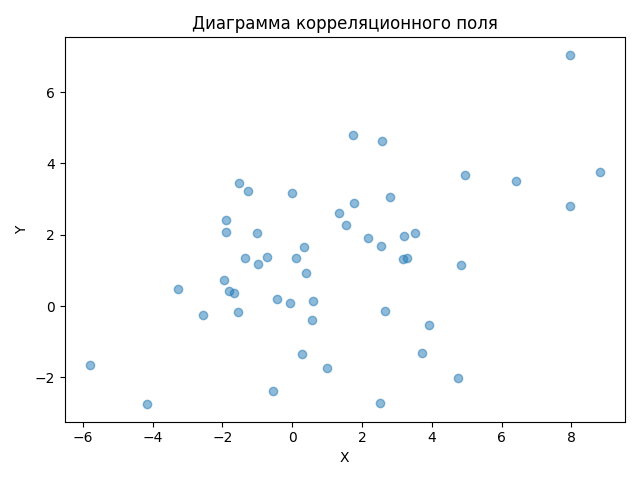
\includegraphics[width=\linewidth]{figures/cor_field}
		\end{center}
	\end{minipage}
\end{figure}

В соответствии с заданием были вычислены:

\begin{itemize}
	\item Коэффициенты линейной регрессии
	\item Коэффициент корреляции
	\item Расчётные значения $\hat{y}_i = a + b \cdot x_i$, $i = \overline{1,n}$
	\item Отклонения $e_i = y_i - \hat{y}_i$, $i = \overline{1, n}$ истинных значений признака от расчётных
	\item Средняя квадратическая ошибка аппроксимации
	\item Значения $t$-статистики для коэффициента корреляции и оценок $a$ и $b$. Также были сделаны выводы о статистической значимости данных коэффициентов.
	\item Доверительные интервалы с уровнем значимости 5\% для параметров $\alpha$ и $\beta$ линейной регрессии
	\item Стандартная ошибка $m_y$ прогноза индвидуального значения
	\item Доверительный интервал полученного прогноза с уровнем значимости 5\%
	
\end{itemize}

Также были построены следующие графики:

\begin{itemize}
	\item График остатков $e$ по отношению к фактору $x$ и по отношению к номеру наблюдения
	
	\begin{figure}[H]
		\begin{minipage}[H]{0.5\linewidth}
			\begin{center}
				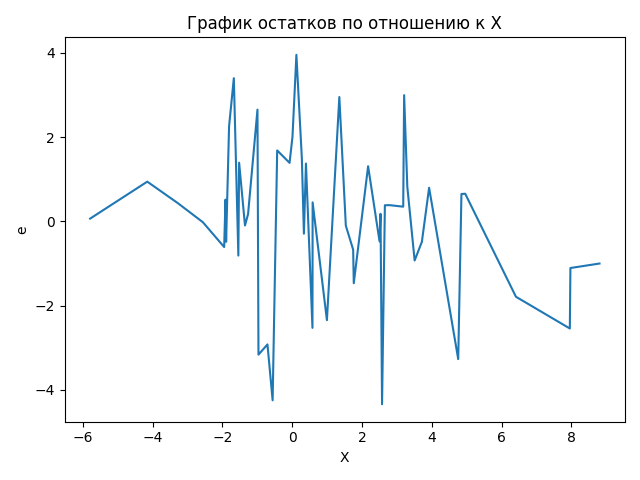
\includegraphics[width=\linewidth]{figures/X_e}
			\end{center}
		\end{minipage}
		\hfill
		\begin{minipage}[H]{0.5\linewidth}
			\begin{center}
				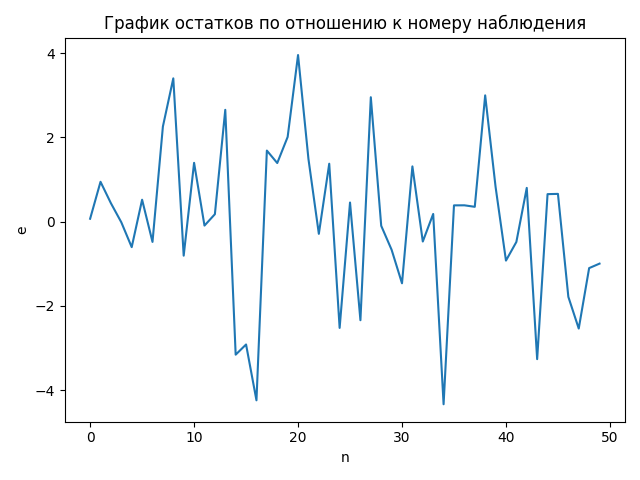
\includegraphics[width=\linewidth]{figures/n_e}
			\end{center}
		\end{minipage}
	\end{figure}

	\item Совместный график корреляционного поля и прямой линейной регрессии:
	
	\begin{figure}[H]
		\begin{minipage}[H]{0.95\linewidth}
			\begin{center}
				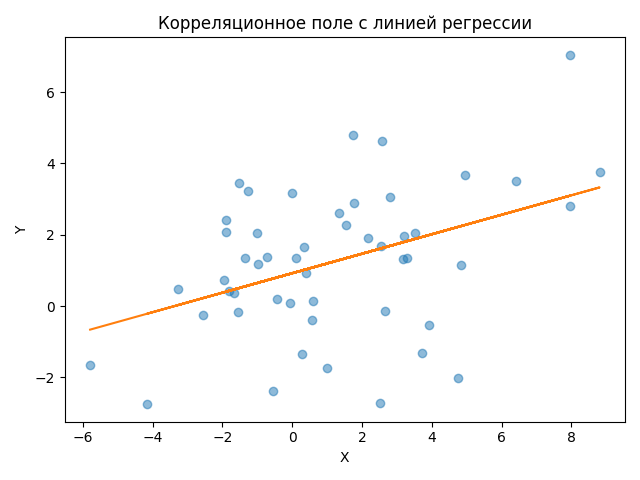
\includegraphics[width=\linewidth]{figures/cor_field_with_reg}
			\end{center}
		\end{minipage}
	\end{figure}

	\item Точечный прогноз $\hat{y}_p = a + b \cdot x_p$, где $x_p$ на 200\% больше, чем средний уровень $\overline{x}$
	
	\begin{figure}[H]
		\begin{minipage}[H]{0.95\linewidth}
			\begin{center}
				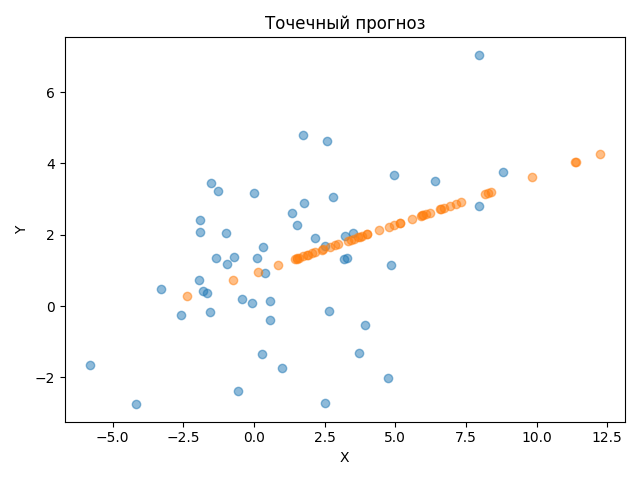
\includegraphics[width=\linewidth]{figures/predict}
			\end{center}
		\end{minipage}
	\end{figure}
	
\end{itemize}

Все вычисленные результаты представлены ниже.

\VerbatimInput{figures/file.txt}